\documentclass{article}
\usepackage{listings}
\usepackage{graphicx}
\author{Yuxiang Chen 5110309783}
\title{Report of Lab5 and Lab6}
\begin{document}
\maketitle
\tableofcontents
\section{The Purpose of This Experiment and My Preparation}
Needless to say, this experiment is mainly based on the Linux, another currently-using operating system. And we have to use hadoop to finish the experiment and learn a method called mapreducing.  This method consists of, as you can see from its name, two parts -- map and reduce. To map is to set up an index of the inputs, and to reduce is just to make a synthesis of the output from the map method. And in this way, we can solve some certain problems.\\
The second part enables us to do some hadoop streaming jobs -- which means we can process more files. Of course, this part also requires the mapreducing method.
\section{The Main Part of the Experiment}
Well, as an introduction of hadoop and probably Linux, this experiment is not very difficult, except for some mistakes we have engaged in when establishing the environment of hadoop. As I have met so many problems when trying to set up my own hadoop, so I decided to use the visual machine the TA had given us.
Of course, there were still some mistakes even though I imitate the steps given in the demo ppt. But to make this report more based on the experiment itself, I will not list all these problems here. And the following are my result of the questions in these ppts.
\subsection{The answer to Mini Problems}
As the first ppt just intends to tell us some basic knowledges of hadoop, so the first part, in my opinion, doesn't need codes written by us. And the only thing we have to do is to get the result of the first problem, copying the command lines. The second mini exercise is just giving us a chance to try some sets of numbers to get the final pi we want.
Here are the results of the problems:
\begin{figure}[htbp]
\centering
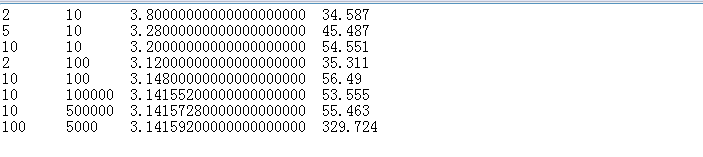
\includegraphics[width=10cm]{000.png}
\caption{total result}
\end{figure}
\begin{figure}[htbp]
\centering

\includegraphics[width=10cm]{001.png}
\caption{the result of 2 and 10}
\end{figure}
\begin{figure}[htbp]
\centering
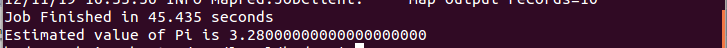
\includegraphics[width=10cm]{002.png}
\caption{the result of 5 and 10}
\end{figure}
\begin{figure}[htbp]
\centering
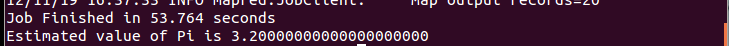
\includegraphics[width=10cm]{003.png}
\caption{the result of 10 and 10}
\end{figure}
\begin{figure}[htbp]
\centering

\includegraphics[width=10cm]{004.png}
\caption{the result of 2 and 100}
\end{figure}
\begin{figure}[htbp]
\centering

\includegraphics[width=10cm]{005.png}
\caption{the result of 10 and 100}
\end{figure}
\begin{figure}[htbp]
\centering
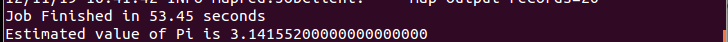
\includegraphics[width=10cm]{006.png}
\caption{the result of 10 and 100000}
\end{figure}
\begin{figure}[htbp]
\centering

\includegraphics[width=10cm]{007.png}
\caption{the result of 10 and 500000}
\end{figure}
\begin{figure}[htbp]
\centering

\includegraphics[width=10cm]{008.png}
\caption{the result of 100 and 5000}
\end{figure}
And the last three pictures are my results of the second Mini problem, and the last result attain the standard TA has given in the ppt files. I try these data just to learn more about the mapreducing method, and I find that the first number, which means the number of times of the experiment, is much more stronger than the second number, which means the number of experiments each time. And this means the more the times of experiments, the bigger the total time of calculating pi.
\subsection{Calculate the Average Length of a Certain Initial Letter}
This part is a little difficult because we are new at this operating system, so there are a lof of trouble at this experiment. However, I managed to solve it by trying so many times to understand what each command line means. And for this experiment, what we have to do is firstly make all the initial letters in their small form and then use the mapreduce method to get the total length of each initial letter, of course, then we can get the average length easily.\\
Here are my mapper codes:
\begin{lstlisting}[language=python,numbers=left,frame=leftline]
#!/usr/bin/env python

import sys
import string
import re

for line in sys.stdin:
    line = line.strip()
    line = re.sub(r'[^a-zA-Z]', ' ', line)
    words = line.split()
    for word in words:
        print '%s\t%s' % (string.lower(word), len(word))

\end{lstlisting}
In this part, I only eliminate all the punctuation in the essay and then spilt them up. And the following are my reduce method:
\begin{lstlisting}[language=python,numbers=left,frame=leftline]
#!/usr/bin/env python

from operator import itemgetter
import sys

current_word = None
current_count = 0
word = None
word_num=0

for line in sys.stdin:
    line = line.strip()
    word, count = line.split('\t', 1)
    try:
        count = int(count)
    except ValueError:
        continue

    if current_word == word[0]:
        current_count += count
        word_num+=1
    else:
        if current_word:
            average=float(current_count)/word_num
            print '%s\t%f' % (current_word, average)
        current_count = count
        current_word = word[0]
	    word_num=1

if current_word == word[0]:
    average=float(current_count)/word_num
    print '%s\t%f' % (current_word, average)

\end{lstlisting}
This part, of course, count the total length of each initial letter and also count the number of words initialed of each letter, then we can get the result we want easily.\\
Here are some pictures of my results:\\
\begin{figure}[htbp]
\centering
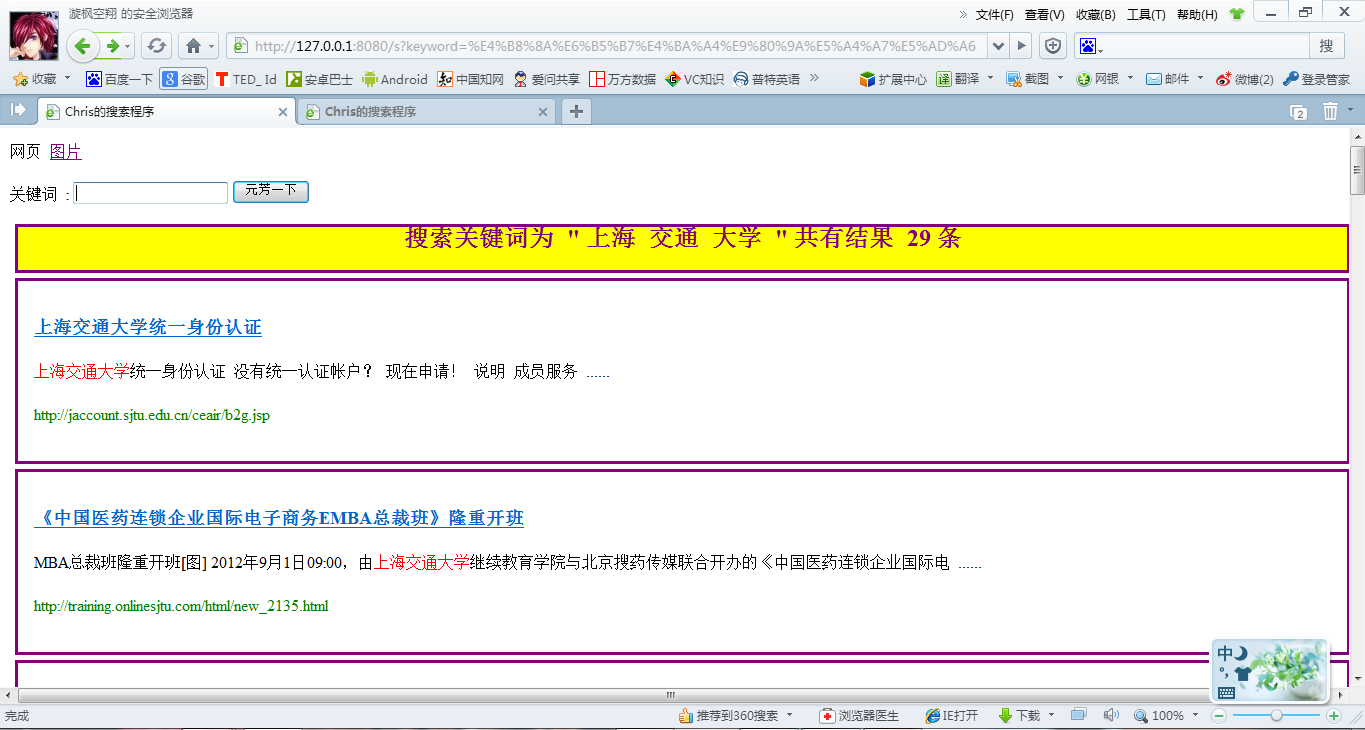
\includegraphics[width=10cm]{6.png}
\caption{the process and command line}
\end{figure}
\begin{figure}[htbp]
\centering
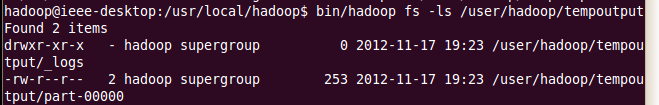
\includegraphics[width=10cm]{7.png}
\caption{the catalog of the output fold}
\end{figure}
\begin{figure}[htbp]
\centering
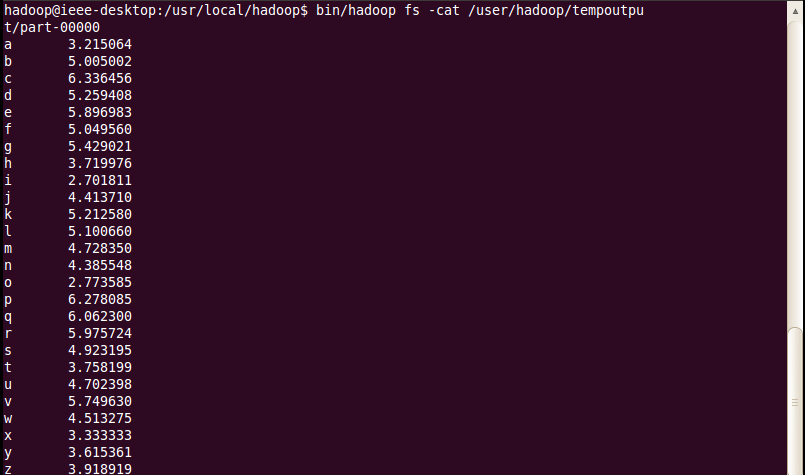
\includegraphics[width=10cm]{4300.png}
\caption{the result of a part of essay 4300}
\end{figure}
\begin{figure}[htbp]
\centering
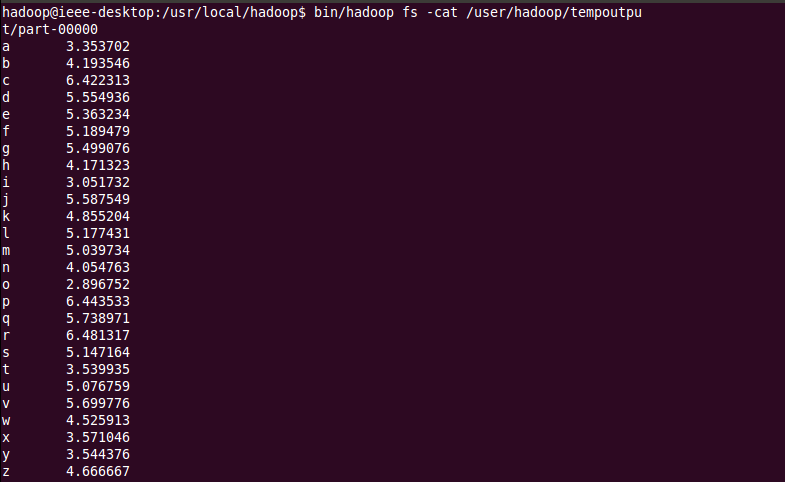
\includegraphics[width=10cm]{5000.png}
\caption{the result of a part of essay 5000}
\end{figure}
\begin{figure}[htbp]
\centering
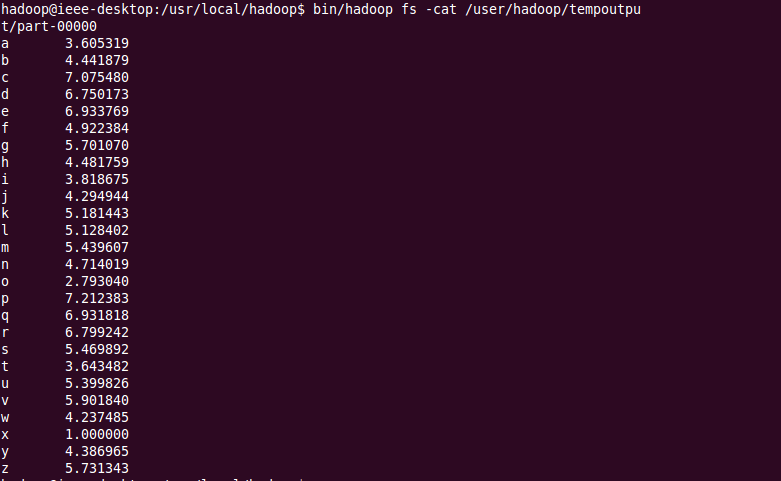
\includegraphics[width=10cm]{20417.png}
\caption{the result of a part of essay 20417}
\end{figure}
\subsection{Getting the PageRank}
This part requires us to get the pagerank of all nodes in a topological graph. And to accomplish this, we need to pass two pieces of information : the links between those nodes and the weight they get from their linking nodes. And what we need to pay attention to is we have to make sure the input and the output are in the same form, since we will have to make the output into a new input in the chaining jobs. And I have been trying for a long time to get a method, with which I can get the relationship(or link-relation) among those nodes in 'mapper' and pass them to 'reducer'. But after so many times of trying, I failed. So I just store their relations as a constant variable in 'reducer'. And we can modify the numbers of nodes, their relationships and alpha(represented with 'a' in my code) in 'reducer'. I decide to store them this way because I think if we have a large number times of experiments, say, 100,000, than if we write a code to get the relationship of the nodes in 'mapper', then it will be executed for also 100,000 times. So if I just store it in the reducer, it can be treated as a strategy of 'getting time in the price of space'.\\
And here are my codes of mapper:
\begin{lstlisting}[language=python,numbers=left,frame=leftline]
#!/usr/bin/env python

import sys

for line in sys.stdin:
    line = line.strip()
    elements = line.split('\t')
    linknodes=eval(elements[2])
    length=len(linknodes)
    node_id=elements[0].strip()
    pr=elements[1]
    link=list()
    just_for_bug=list()
    just_for_bug.append(node_id)
    just_for_bug.append(0)
    print node_id,'\t',just_for_bug
    for l in linknodes:
    	average=float(pr)/length
    	assemble=list()
    	assemble.append(node_id)
    	assemble.append(average)
        print l,'\t',assemble

\end{lstlisting}
In the former part, I just pass the information of every node into the reducer from the input, and the reducer is as follows:
\begin{lstlisting}[language=python,numbers=left,frame=leftline]
#!/usr/bin/env python

from operator import itemgetter
import sys

current_node = None
current_pr = 0
node = None
a=0.85
num=4
flag=0
total_link=[[2,3,4],[3,4],[4],[2]]

# input comes from STDIN
for line in sys.stdin:
    # remove leading and trailing whitespace
    line = line.strip()

    # parse the input we got from mapper.py
    line= line.split('\t')
    node=line[0]
    add_list=line[1]
    add_list=eval(add_list)
    add_pr=add_list[1]

    try:
        add_pr = float(add_pr)
    except ValueError:
        continue

    if current_node == node:
        current_pr += add_pr
    else:
        if current_node:
    	    final_pr=a*current_pr+(1-a)/num
    	    final_pr=float('%.4f' % final_pr)
            print current_node,'\t',final_pr,'\t',total_link[flag]
    	    flag+=1
        current_node = node
        current_pr = add_pr

# do not forget to output the last word if needed!
if current_node == node:
    final_pr=a*current_pr+(1-a)/num
    final_pr=float('%.4f' % final_pr)
    print current_node,'\t',final_pr,'\t',total_link[flag]

\end{lstlisting}
In this part, I just calculate the rank of each node and then given them the same form as the input file and then output them. And to make the form tidier, I make the result shown with four numbers after the point in the decimal. Meanwhile, to get the result we want being output in a file, I change the last sentence of the 'batch for pageRank.sh', which is as follows:
\begin{lstlisting}[language=python,numbers=left,frame=leftline]
#/bin/bash

command='bin/hadoop jar contrib/streaming/hadoop-0.20.2-streaming.jar -file /home/experiments/src/mapper.py -mapper /home/experiments/src/mapper.py -file /home/experiments/src/reducer.py -reducer /home/experiments/src/reducer.py'
mv='bin/hadoop fs -mv '
rm='bin/hadoop fs -rmr '
cp='bin/hadoop fs -copyToLocal '
ct='bin/hadoop fs -cat'
function func()
{
for ((i=1;i<$1+1;i++));
do
    echo "Processing $i"
    eval "$command -input $2/* -output tempoutput"
    eval "$rm $2"
    eval "$mv /user/hadoop/tempoutput $2"
done
}
func $1 $2
#eval "$cp $2/* /home/experiments/output/result.txt"
eval "$ct $2/part-* > /home/hadoop/result.txt"
\end{lstlisting}
Thus we can find the final result at 'result.txt'. As I have said, to save time, I just let the code run for three times to get a demo result because the slow visual machine...\\
\begin{figure}[htbp]
\centering
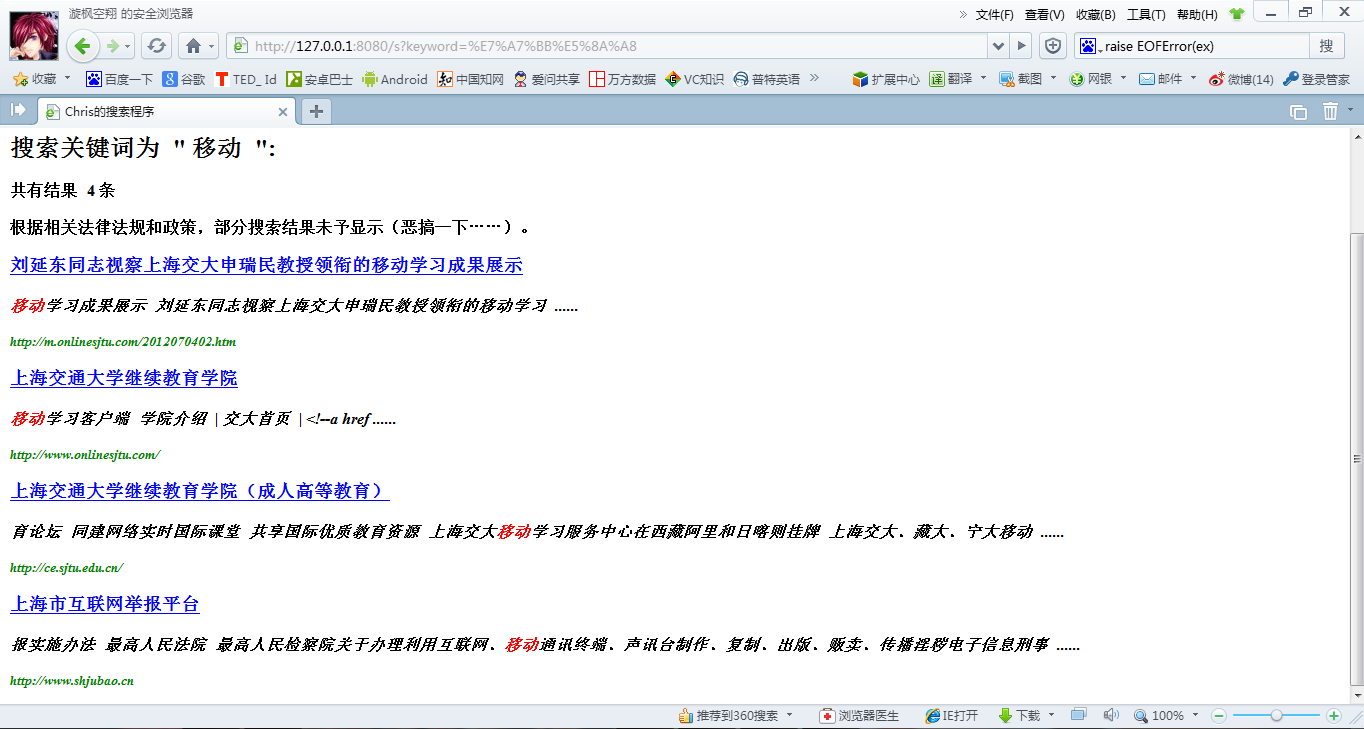
\includegraphics[width=10cm]{4.png}
\caption{Processing 1}
\end{figure}
\begin{figure}[htbp]
\centering
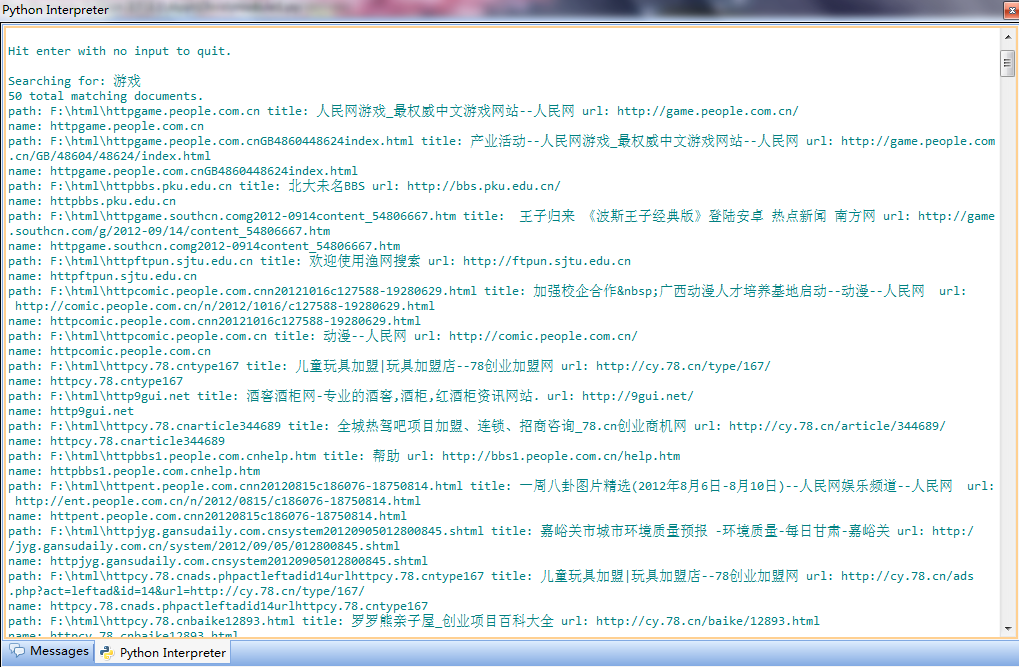
\includegraphics[width=10cm]{5.png}
\caption{Processing 2}
\end{figure}
\begin{figure}[htbp]
\centering
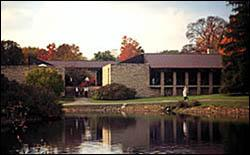
\includegraphics[width=10cm]{1.png}
\caption{Processing 3}
\end{figure}
\begin{figure}[htbp]
\centering
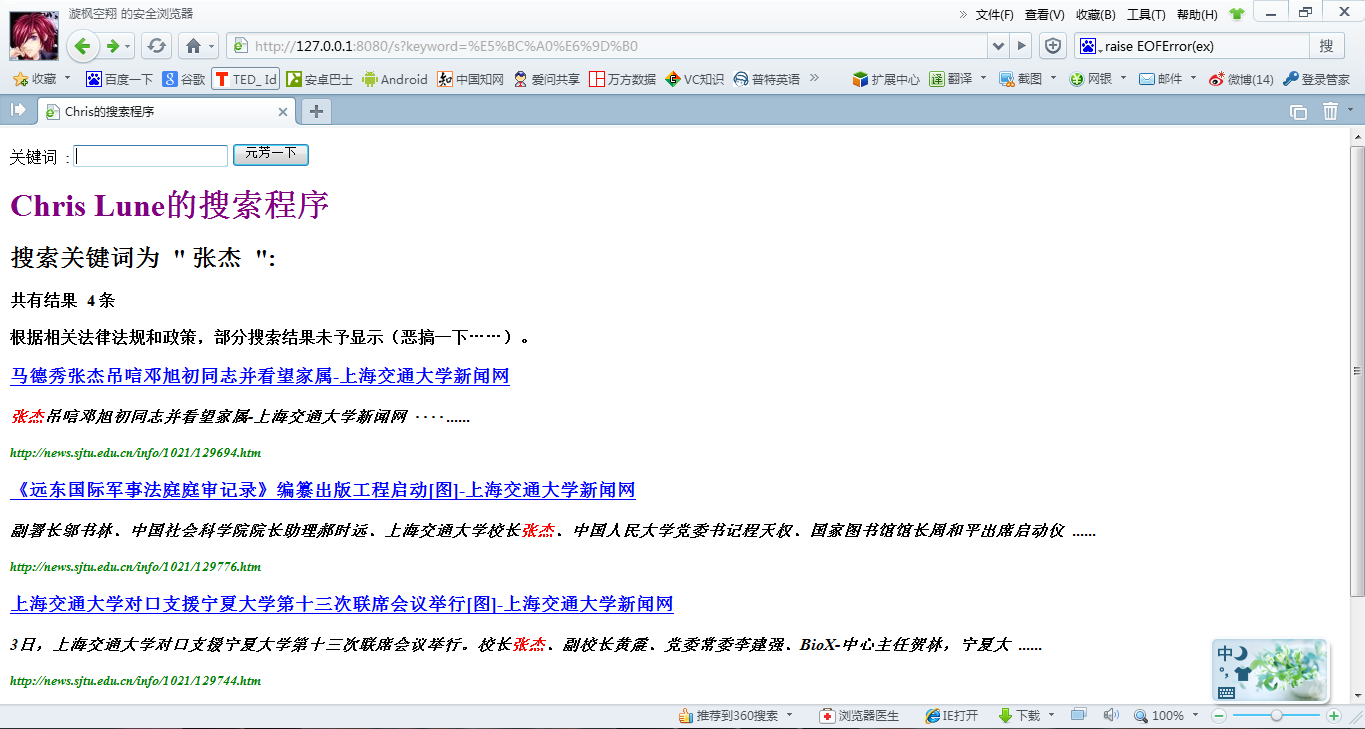
\includegraphics[width=10cm]{3.png}
\caption{the input file}
\end{figure}
\begin{figure}[htbp]
\centering

\includegraphics[width=10cm]{2.png}
\caption{the outcome of the first round}
\end{figure}
\begin{figure}[htbp]
\centering
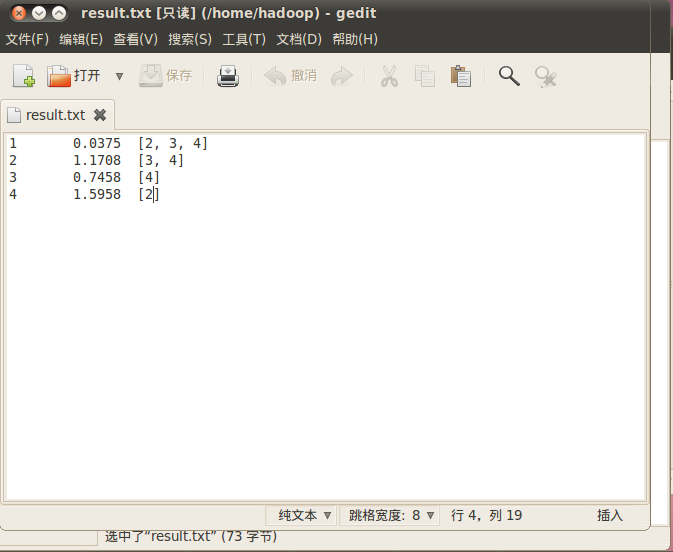
\includegraphics[width=10cm]{0.png}
\caption{the outcome of the third round}
\end{figure}
\section{The Problems I Met and My Thoughts}
In the experiment, there're just to many problems. And I'll only take the typical ones.\\
First, at the 'initial-letter-length finding' part, I have some trouble eliminating the punctuation of the essay, then I searched for it and solve it using the regular expression:\\
\begin{lstlisting}[language=python,numbers=left,frame=leftline]
    line = line.strip()
    line = re.sub(r'[^a-zA-Z]', ' ', line)
\end{lstlisting}
And then at the 'pagerank' part, I try to give the decimals four numbers after the point, and here is how I solve it at last:\\
\begin{lstlisting}[language=python,numbers=left,frame=leftline]
final_pr=float('%.4f' % final_pr)
\end{lstlisting}
Of course, I said earlier that I can't pass the relationship to 'reducer' at first in the 'pagerank' part, and I also give my solution to the problem in the former section.\\
I think the mapreduce method is just like building lots of threads and giving each thread a certain job, which makes the problem easier and faster. Meanwhile, I'm pretty interested in the pagerank calculating method, because I think with which, we can make our searching engine more organized when giving out the searching results. And we can also give every page a suitable position in the final output page in terms of their ranks.
\end{document}
